\chapter{范畴, 函子, 自然变换}\label{Chap.Cat.Funct.NormTranf}
% MARK: Chpt: 范畴
\says{现代数学常出现\squarebrace{自然性}现象.}{Samuel Eilenberg 和 Saunders Mac Lane,\\``Natural isomorphisms in group theory''}{TODO}

\par 对 Abel 群 \(G\), Abel 群 \(H\) 的\textbf{群扩张} 为群 \(E\), 嵌入 \(G\hookrightarrow E\) 为正规子群, 满同态 \(E\twoheadrightarrow H\) 将 \(H\) 表示为商群 \(E/G\). 上述数据常以群同态图表示:\[
    \begin{tikzcd}
        0 \ar[r] & G \ar[r] & E \ar[r] & H \ar[r] & 0 
    \end{tikzcd}\footnotemark
\]\footnotetext{结尾的 0 不提供额外信息, 但开头的 0 断定了映射 \(G\to E\) 是嵌入, 而这一嵌入映射又断定了其后的 \(E\to H\) 为满射. 更准确地说, 这些群同态给出的序列\textbf{正合}, 也就是说, 前一个同态的像总恰为后一个同态的核.}
存在同构 \(E\cong E'\), 且其\textit{交换}对 \(G\) 的嵌入与商映射到 \(H\)时, 认为 \(G\) 和 \(H\) 的一对群扩张 \(E\) 和 \(E'\) 等价, 这一叙述某种意义上将于\chptref{Sec.The.art.if.the.diagram.chase}. \(H\) 的 \textit{Abel} 群扩张等价类由 \(G\) 定义 Abel 群 \(\Ext(H,G)\).
\par 于 1941 年, Saunders Mac Lane 在 Michigan 大学演讲时, 针对素数 \(p\) 证明了
        \[\Ext\left(
            \left[
                \dfrac{1}{p}
            \right]
                \middle/
            \mathbb{Z},\mathbb{Z}
        \right) \cong \mathbb{Z}_p,\] 
即 \(p\)--进整数群, 其中, \(\left[\dfrac{1}{p}\right]\bigg/ \mathbb{Z}\) 为 Pr\"ufer \(p\)--群. 他向 Samuel Eilenberg 解释这一结果时忘记了自己的演讲过程, Eilenberg 回想该计算结果为 \(p\)--进螺线 3 维球面补空间的同调, 由一个实心圆环序列的无穷交构成的空间, 每个环在前一个环内绕 \(p\) 次. 在梳理其中联系时, 二人发现了一个定理, 代数拓扑领域现在称其作\textbf{万有系数定理}, 该定理将同调 \(H_*\) 和上同调群 \(H^*\) 与一个空间 \(X\) 通过群扩张\cite{ML05}
\begin{equation}\label{Eq:0.Ext.Hn.Hom.0}
    0\rightarrow\Ext\left(H_{n-1}(X),G\right)\rightarrow H^n(X,G)\rightarrow\Hom\left(H_n(X),G\right)\rightarrow 0
\end{equation}
联系了起来.
\par 为获得万有系数定理更泛用的构造, Eilenberg 和 Mac Lane 不得不用证明一些表以群扩张的 Abel 群同构, 其能够扩张至经由极限或余极限构造的空间. 诚则确然, 正因图 \eqref{Eq:0.Ext.Hn.Hom.0} 述同态皆\textit{自然}于拓扑空间间的连续映射.
\par \squarebrace{自然}一词在数学家口中意味着\squarebrace{不依赖任选而定义}. 例如, 定义有限维向量空间 \(V\) 及其\textbf{对偶}间的同构, 即由从 \(V\) 至基域 \(\mathbb k\) 的线性映射构成的向量空间, 依赖于基的选择; 又如, 存在从 \(V\) 至其双对偶间的同构, 其定义不依赖基: 故而仅后述之映射定义\textit{自然}.
\par 为证明其特定群同构族扩张至极限和余极限, Eilenberg 和 Mac Lane 设法给出非正式概念\squarebrace{自然性}在数学上精确的定义, 为此他们引入了\textit{自然变换}, 上述情形下 Abel 群的同态平行总和; 为描述自然变换的源与目标, 又引入了\textit{函子}\footnote{群论中, 函子与自然同构于 1942 年的一份文献 \cite{EM42b} 内有简短介绍.}; 而为普适定义函子的源和目标, 又引入\squarebrace{范畴}这一概念: 上述工作称以\squarebrace{自然等价的一般理论}\ref{EM45}, 在 1945 年发表, 是为范畴论的诞生日.
\par 范畴与函子最开始作为辅助记号提出, 这是因为自然性这一概念确需精确定义, 而现在, 其本身亦足够有趣、足够重要. 范畴论提出数学对象研究时的一种不同视角, 即不再过分关注对象本身, 而把更多精力放在对象间的关系上. 函子能够翻译数学对象的一种形式到另一种形式, 应用更为直接, 例如, Brouwer 不动点定理翻译拓扑中似乎棘手的问题为代数中的平凡问题 (即 \(0\ne1\)), 这正是我们目前转向的主题.
\par 范畴将于 \chptref{111} 以两种形式介绍: 其一作为宇宙分类数学对象, 其二其自身亦视作数学对象. 前者用于譬如定义更广义的\textit{同构}概念, 使其能够专门用于各式各样的数学对象. 后者则引出, 那些公理定义下, 范畴必自对偶.\footnote{确然如此, 对于射影平面几何, 其对偶性可确切述作公理化其结构的一阶逻辑定理.} 因此, 正如 \chptref{1212} 所探索的, 从那些公理开始, 对关于所有范畴的定理, 其任何证明均具一对偶证明于对偶定理, 这一对偶定理由称作\squarebrace{反转所有箭头}的句法过程得到.
\par 函子和自然变换于 \chptref{1133} 和 \chptref{1144} 引入, 其中举例, 旨在阐明个中用语及实际应用. 范畴论记号\textit{同构 (Isomorphism)、左消态射 (Monomorphism)、右消态射 (Epimorphism)} 在特定函子类中不变, 尤其包括\textit{范畴等价}, 将于 \chptref{1155} 引入. 切要剖之, 有了范畴等价, 得以精准表达某两种类型数学对象间\squarebrace{等同}的直觉: 矩阵范畴和有限维向量空间范畴间的等价, 相当于高中和大学的线性代数间的等价.
\par 除提供新的语言以描述新兴数学现象, 范畴论亦引入新的证明工具: 图索法 (diagram chase). 著作 \cite{ES52} 的导言中展示, \textit{交换图}作为\squarebrace{新的证明工具}之一, 正逐渐成为同伦论的公理化处理手段. 图索法这一工具将介绍于 \chptref{1166}, 然后应用于 \chptref{1177} 以构建新的自然变换为给定自然变换的\textit{纵复合}或\textit{横复合}.

\section{抽象范畴与具体范畴}
% MARK: 抽象具体范畴
\says{为所有数学理论构建可能平台: 只要这个理论有\textit{名词}和\textit{动词}, 即对象和态射, 且对态射来说有明确的复合, 那该理论则显然理应归类为范畴.}{Barry Mazur, ``When is one thing equal to some other thing?''}{Maz08}
\begin{definition}\label{Def:Category}
    \textbf{范畴}为含有
        \begin{itemize}
            \item \textbf{对象 (object)}的总体 (collection) \(X,Y,Z,\dots\)
            \item \textbf{态射 (morphism)}的总体 \(f,g,h,\dots\)
        \end{itemize}
    并使得
        \begin{itemize}
            \item 任意态射均唯定其\textbf{域 (domain)} 与\textbf{上域 (codomain)} 对象; 记号 \(f\colon X\to Y\) 表示 \(f\) 为有域 \(X\) 与上域 \(Y\) 的态射.
            \item 任意对象均拥有唯定\textbf{恒等态射} \(1_x\colon X\to X\).\footnote{译注: 这里不意味着任意态射 \(f\colon X\to Y\), 当 \(X=Y\) 时有 \(f=1_X\). 用后文提到的记号, 这里更合理的说法是, 对任意对象 \(X\), 均存在唯定幺态射 \(1_X\in\Hom(X,X)\).}
            \item 对任意态射对 \(f,g\), 其中 \(f\) 的上域等于 \(g\) 的域, 总存在唯定\textbf{复合态射 (composite morphism)}\footnote{若至混淆, 则记号 \(g\cdot f\) 不可简写如上.} \(gf\), 其域为 \(f\) 的域, 上域为 \(g\) 的上域, 即\footnote{译注: 更明朗的写法:\begin{align*}(\cdot)\colon\Hom(X,Y)\times\Hom(Y,Z) & \to \Hom(X,Z)\\(f,g)\kern3em&\mapsto gf=g\cdot f\end{align*}}:\[
                f\colon X\to Y,\quad g\colon Y\to Z\qquad\rightsquigarrow\qquad gf\colon X\to Z.\]
        \end{itemize}
    的二元组. 其资料受制于如下两公理:
        \begin{itemize}
            \item 对任意 \(f\colon X\to Y\), 恒有 \(1_Yf=f1_X=f\).
            \item 对任意可复合的态射三元组 \(f\), \(g\), \(h\), 复合结果 \(h(gf)\) 和 \((hg)f\) 认为等同, 均记作 \(hgf\).\[
                    f\colon X\to Y,\quad g\colon Y\to Z,\quad h\colon Z\to W\qquad\rightsquigarrow\qquad hgf\colon X\to W.
                \]
        \end{itemize}
    亦即, 态射复合可结合, 存在幺, 其幺态射即保持双边幺的恒等态射.
\end{definition}
\begin{remark}\label{Rem:CategoryOtherDfntn}
    范畴的对象与恒等态射存在双射对应, 且该对应唯定, 因为他们对态射复合保持双边幺. 故可定义范畴为态射总体, 拥有部分定义的复合运算, 存在特定态射用以识别复合对并保持双边幺, 参见 \cite{Ehr65} 或 \cite{FS90}. 但实践中, 同时指定对象和态射并不困难, 本书亦将如此处理.
\end{remark}
\par 传统上用其对象命名范畴; 同时通常来说, 更倾向于使用那些随之而来的结构保持态射更清晰的选择. 然而这一做法有违范畴论的基本哲学: 数学对象理应总与其间的态射一并考虑. 根据注解 \ref{Rem:CategoryOtherDfntn}, 态射的代数决定了范畴, 故而在对象和态射之间, 后者更具首要地位.

\begin{example}\label{Expl:Concrete.Category}
    许多数学对象可组装为范畴.
    \begin{enumerate}[label={(\roman*)}, ref = {(\roman*)}]
        \item 集合范畴 \(\cat{Set}\) 以集合为对象, 拥有具体域、上域的函数为态射.
        \item 拓扑空间范畴 \(\cat{Top}\) 以拓扑空间为对象, 连续函数为态射.
        \item \(\cat{Set}_*\) 和 \(\cat{Top}_*\) 以指定基点的集合或拓扑空间为对象, 保持基点的 (连续) 函数为态射.
        \item 群范畴 \(\cat{Group}\) 以群为对象, 群同态为态射. 此例赋予\squarebrace{态射}这一通用术语以抽象范畴的数据. 环范畴 \(\cat{Ring}\) 由交换幺环和环同态构成, 域范畴 \(\cat{Field}\) 由域和域同态构成, 皆有相近定义.
        % \item 给定幺环 \(R\) (未必交换), 左 \(R\)--模范畴 \(\cat{Mod}_R\) 由左 \(R\)--模与模同态构成. 当环实为域 \(\mathbbpdf k\) 时,该范畴进一步为线性空间范畴 \(\cat{Vect}_\mathbbpdf k\); 而为 \(\mathbb Z\) 时进一步为 Abel 范畴 \(\cat{Ab} =\cat{Mod}_\mathbb Z\), 因为 \(\mathbb Z\)--模实际就是 Abel 群.
        \item 给定幺环 \(R\) (未必交换), 左 \(R\)--模范畴 \(\cat{Mod}_R\) 由左 \(R\)--模与模同态构成. 当环实为域 \(\mathbbpdf{\mathrm k}\) 时,该范畴进一步为线性空间范畴 \(\cat{Vect}_{\mathbbpdf{\mathrm k}}\); 而为 \(\mathbb Z\) 时进一步为 Abel 范畴 \(\cat{Ab} =\cat{Mod}_{\mathbb Z}\), 因为 \(\mathbb Z\)--模实际就是 Abel 群.
        \item 图范畴 \(\cat{Graph}\) 以图为对象, 以图同态 (将顶点映到顶点, 边映到边, 同时保持连接关系的函数) 为态射. 另有有向图范畴 \(\cat{DirGraph}\), 以有向图为对象, 其边画作箭头, 而态射则为有向图同态, 即必保持边的方向.
        \item 流形范畴 \(\cat{Man}\) 以光滑流形 (即无穷阶可微) 为对象, 光滑映射为态射.
        \item 可测空间范畴 \(\cat{Mea}\) 以可测空间为对象, 可测函数为态射.
        \item 偏序集范畴 \(\cat{Poset}\) 以偏序集为对象, 保序函数为态射.
        \item \(\cat{Ch}_R\) 以 \(R\)--模的链复形为对象, 链同态为态射.
        \item 对任意指配有常数、函数、关系符的字符集 \(\sigma\), 以及所有在 \(\sigma\) 相关的一阶语言中良构的语句, 构成集 \(\mathbb T\), 可有模型范畴 \(\cat{Model}_{\mathbb T}\), 其对象为\textit{模型} \(\mathbb T\) 的 \(\sigma\)--结构, 亦即配备了满足公理 \(\mathbb T\) 的相应常数、关系、函数的集合. 而态射即通常的保持指定常数、关系、函数的映射. 这一范畴的特例包括前述的 (iv), (v), (vi), (ix),~(x).
    \end{enumerate}
\end{example}
\par 上述即\textit{具体范畴 (concrete category)} 的全部例子, 即对象基于集合, 而态射为这些对象背后的集合间的函数, 尤其是\squarebrace{结构保持}态射. 具体范畴有一个更精确的定义, 于 \ref{114417} 给出. 此外, \squarebrace{抽象}范畴亦很广泛:
\begin{example}\label{Expl:Abstract.Category}
    \ \begin{enumerate}[label={(\roman*)}, ref = {(\roman*)}]
        \item 给定幺环 \(R\), 范畴 \(\cat{Mat}_R\) 以正整数为对象, 而其从 \(n\) 到 \(m\) 的态射集为值在 \(R\) 中的那些 \(m\times n\) 矩阵构成的集. 态射复合由矩阵乘法\[
            n\xrightarrow{A}m,\quad m\xrightarrow{B}k\qquad\rightsquigarrow\qquad n\xrightarrow{B\cdot A} k
        \]
        完成, 其中单位矩阵体现为单位态射.
        \item 一个群 \(G\) (或更宽泛地说, 一个幺半群) 定义一个范畴 \(\cat BG\), 仅具唯一对象. 群元作为该范畴的态射, 分别代表该唯一对象上的不同自同态, 而态射复合即群乘法. 幺 \(e\in G\) 即为单位态射.
            \begin{center}
                \centering
                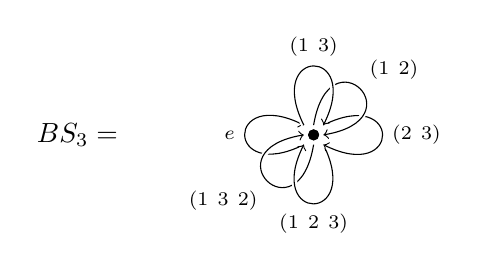
\begin{tikzpicture}
                    \node(BS3)at(0,0){$\cat BS_3=$};
                    % 左侧 S_3
                    \node(dot)at(3,0){\ };
                    \fill (dot) circle [radius=2pt];
                    \draw[color = white, line width = 2pt] (dot.south west) .. controls +(-1,-0.5) and +(-1,0.5) .. (dot.north west);
                    \draw[->] (dot.south west) .. controls +(-1,-0.5) and +(-1,0.5) .. node[left,midway] {{$\scriptstyle e$}} (dot.north west);
                    \draw[color = white, line width = 2pt] (dot.south) .. controls +(-0.2,-1.2) and +(-1.2,-0.2) .. (dot.west);
                    \draw[->] (dot.south) .. controls +(-0.2,-1.2) and +(-1.2,-0.2) .. node[below left,midway] {$\scriptstyle (1\ 3\ 2)$} (dot.west);
                    \draw[color = white, line width = 2pt] (dot.south east) .. controls +(0.5,-1) and +(-0.5,-1) ..  (dot.south west);
                    \draw[->] (dot.south east) .. controls +(0.5,-1) and +(-0.5,-1) .. node[below,midway] {$\scriptstyle (1\ 2\ 3)$} (dot.south west);

                    % 右侧 S_3 的中心对称
                    \node(dot2) at (3,0) {\ };
                    \fill (dot2) circle [radius=2pt];
                    \draw[color = white, line width = 2pt] (dot2.north east) .. controls +(1,0.5) and +(1,-0.5) .. (dot2.south east);
                    \draw[->] (dot2.north east) .. controls +(1,0.5) and +(1,-0.5) .. node[right,midway] {{$\scriptstyle (2\ 3)$}} (dot2.south east);
                    \draw[color = white, line width = 2pt] (dot2.north) .. controls +(0.2,1.2) and +(1.2,0.2) .. (dot2.east);
                    \draw[->] (dot2.north) .. controls +(0.2,1.2) and +(1.2,0.2) .. node[above right,midway] {$\scriptstyle (1\ 2)$} (dot2.east);
                    \draw[color = white, line width = 2pt] (dot2.north west) .. controls +(-0.5,1) and +(0.5,1) ..  (dot2.north east);
                    \draw[->] (dot2.north west) .. controls +(-0.5,1) and +(0.5,1) .. node[above,midway] {$\scriptstyle (1\ 3)$} (dot2.north east);
                \end{tikzpicture}
            \end{center}
            \item 偏序集 \((\cat P,\le)\) (或更一般地说, 预序集) 可视作范畴. \(\cat P\) 的元素即范畴的对象, 而总存在唯一一个态射 \(x\to y\) 当且仅当 \(x\le y\). 偏序关系或者说预序关系 \(\le\) 的传递性蕴含所需态射复合的存在性, 自反性蕴含单位态射的存在性.
            \item 特别地, 任意序数 \(\alpha=\{\beta|\beta<\alpha\}\) 均定义一个范畴, 其对象为那些比之小的序数. 例如, \(\mathbbpdf0\) 为无任何对象或态射的零范畴, \(\mathbbpdf1\) 为仅有一个对象且仅有单位态射的平凡范畴,\footnote{译注: 这里说仅含单位态射, 并非\squarebrace{自然}, 而仅为规定, 反例见前文 \(\cat BG\).}\ \(\mathbbpdf2\) 则为有两个对象, 同时除单位态射外有一个非单位态射的范畴, 传统上描摹作 \(0\to1\). \(\mathbbpdf{\upomega}\) 为\textit{由图}\[
                \begin{tikzcd}
                    0\ar[r]&1\ar[r]&2\ar[r]&3\ar[r]&\cdots
                \end{tikzcd}    
            \]\textit{自由生成}的范畴, 其中, 任意非单位态射均可唯一分解为上示图中态射的复合. 自由生成的精准定义由例 \ref{441113} 给出.
            \item 集合本身亦可视作范畴, 以集合的元素作为对象, 而态射仅有必需的单位态射. 称某范畴\textbf{离散}当且仅当所有态射均为单位态射.
            \item \(\cat{Htpy}\), 类似 \(\cat{Top}\), 以拓扑空间为对象, 但对象为连续映射的同伦类. 而 \(\cat{Htpy}_*\) 须额外指定基空间、基连续映射的基点保持同伦类.
            \item \(\cat{Measure}\) 以可测空间为对象. 而态射选择为可测函数的等价类, 使得平行的一对函数等价, 当其域的差异为零测集.
    \end{enumerate}
\end{example}
\par 上述种种, 道尽范畴论之哲学. 例 \ref{Expl:Concrete.Category} 所陈范畴表明数学对象理应连带期间的态射一起探讨, 而列诸 \ref{Expl:Abstract.Category} 者, 又说明态射并非总是函数.\footnote{Reid 的 \textit{Undergraduate algebraic geometry} (《本科代数几何》) 强调, 态射并非总为函数, 原文\cite[p. 4]{Rei88}:\begin{quote}
    \squarebrace{不认可该点的学生建议立即放弃, 转而修读一门范畴论阅读课程.}
\end{quote}} 范畴的态射亦称\textbf{箭头}或\textbf{映射}, 尤其是在例 \ref{Expl:Concrete.Category} 或 \ref{Expl:Abstract.Category} 的背景下.
\begin{remark}
    Russell 悖论蕴含, 没有一个元素为\squarebrace{所有集合}的集合, 此亦定义 \ref{Def:Category} 中采用模糊的\squarebrace{总体}一词之所咎. 事实亦如此, 例 \ref{Expl:Concrete.Category} 中的所有例子, 其对象总体均非集合. Eilenberg 和 Mac~Lane 如下处理这一潜在漏洞:
        \begin{quote}
            ... 整个范畴的概念本质上仅是辅助概念; 我们将基本概念本质上放在\textit{函子}与自然变换上... 范畴的想法仅仅出于每个函数应有固定的类作为定义域和像而必须, 对范畴而言则表现为函子的定义域和像. 所以说范畴这个概念完全可以摒弃, 而尝试构建一个更符直觉的起点, 这里面像\squarebrace{\(\Hom\)}这样的函子就不定义在\squarebrace{所有}群的范畴上,  而仅仅基于可能给定的每个特定的群对. \cite{EM45}
        \end{quote}
    我们面临如此的集合论问题, 定义范畴概念后, 随着范畴理论发展得更远, 这一问题也会随之越发复杂. 基于这等因素, 范畴论学家的常见做法是在 Zermelo-Fraenkel 集合论公理系统的一个扩张里工作, 拥有额外的一些公理去区分\squarebrace{大集合}和\squarebrace{小集合}, 或者集合和类. 为范畴论寻觅最实用的集合论基础, 这一主题亦很迷人, 但很不幸, 这将离开我们的主题太久时间去探索.\footnote{预印本 \cite{Shu08} 给出了激动人心的概述, 不过建议学完本书第 1---4 章后再去阅读.} 相反, 我们把这个问题压到箱底吧, 并不是说这些问题不重要或者无趣, 只是因为其太分散手头任务的注意力了.\footnote{如果不得已必须处理, 假设存在\textbf{不可达基数}的可数序列, 即不可数基数, 它们\textbf{正则}且\textbf{强极限}. 一基数 \(\kappa\) \textbf{正则}, 若所有少于 \(\kappa\) 的基数之并亦小于 \(\kappa\). 而 \(\kappa\) \textbf{强极限}, 若 \(\lambda<\kappa\) 蕴含 \(2^\lambda<\kappa\). 不可达是指小于 \(\kappa\) 的集合在幂集运算与 \(\kappa\)--小并运算下封闭. 若 \(\kappa\) 不可达, 则 von Neumann 层次的 \(\kappa\) 阶段, 即秩小于 \(\kappa\) 的集合之集 \(V_\kappa\), 是带选择公理的 Zermelo-Fraenkel 集合论 (ZFC) 的一个模型; 集合 \(V_\kappa\) 是一个 \textit{Grothendieck 宇宙}. 假设存在一个不可达基数的可数序列, 即可在 \(V_\kappa\) 内部\squarebrace{使用集合论}, 而后根据需要随时扩大宇宙.
    \par 若 ZFC 一致, 那么该公理系统无法证明不可达基数的存在性, 甚至无法证明假设的一致性 (根据 G\"odel 不完备性定理). 尽管如此, 从大基数公理的层垒观点来看, 不可达基数的存在性假设相对比较温和.}
\end{remark}
\par 出于刚刚提及的理由, 有必要介绍用以描述范畴大小的形容词.
\begin{definition}
    称范畴\textbf{小}, 当且仅当其态射总体不超出集合大小.
    \par 由注解 \ref{Rem:CategoryOtherDfntn}, 小范畴的对象总体不超出集合大小. 若 \(\cat{C}\) 是小范畴, 则有映射\[
    \begin{tikzcd}
        \Mor\cat C \ar[r, yshift=.5em, "{\rm dom}"] \ar[r, yshift=-.5em, "{\rm cod}"swap] & \Ob\cat C \ar[l, "{\rm id}"description]
    \end{tikzcd}\]
    递送态射至其域和上域, 而递送对象至其单位态射.
\end{definition}
\par 例 \ref{Expl:Concrete.Category} 中的范畴均非小, 其中每个范畴均携有太多对象. 但\squarebrace{局部而论}, 它们类似于小范畴, 具体陈述如下:
\begin{definition}
    范畴称\textbf{局部小}, 若对所有对象对, 其间的态射总体不超过集合大小.
\end{definition}
\par 对局部小范畴, 从 \(X\) 到 \(Y\) 的所有态射这一总体习惯上记作\footnote{Mac Lane 赞同 Emmy Noether 所强调的同态在抽象代数中的重要性, 尤其是商群上的同态, 在 Noether 第一同构定理中起了很大作用. 在他回忆中, 箭头记号首次出现于 1940 年, 可能要归因于 Hurewicz \cite{ML88}. 记号 \(\Hom(X,Y)\) 则首次现身于文献 \cite{EM42a}, 用于表示一对 Abel 群间的同态集.}%
\begin{equation}\label{Eq:Locally.Small.Category}
    \cat C(X,Y)\qquad\text{或}\qquad \Hom(X,Y)
\end{equation}%
局部小范畴中, 一对给定对象间的态射集通常称作 \textbf{Hom--集}, 无论其是否任何特定种类的\squarebrace{同态}集. 鉴于 (\ref{Eq:Locally.Small.Category}) 中的记号的确方便, 尽管有时那些指定始终的态射总体大于集合, 亦用上述形式表记之.
\par 给定范畴会提供一个背景, 得以回答:\squarebrace{一物何时同乎另一物?}在数学的几乎任何地方, 以精确的范畴式定义视同一范畴内同构两对象\squarebrace{相同}, 下面介绍同构:
\begin{definition}\label{Def:Isomorphism}
    范畴中, 称态射 \(f\colon X\to Y\) 为\textbf{同构 (Isomorphism)}, 若存在态射 \(g\colon Y\to X\) 使得 \(gf=1_X\) 且 \(fg=1_Y\). 此时称 \(X\) 和 \(Y\) 互为同构, 记作 \(X\cong Y\).
    \par \textbf{自态射 (endomorphism)} 即域与上域相同的态射, 而同构的自态射即称\textbf{自同构 (automorphism)}.
\end{definition}
\begin{example}\label{Expl:Isomorphism}
    \ \begin{enumerate}[label=(\roman*)]
        \item \(\cat{Set}\) 中, 同构即\textbf{双射}.
        \item \(\cat{Group}\), \(\cat{Ring}\), \(\cat{Field}\), \(\cat{Mod}_R\) 中, 同构即双射同态.
        \item \(\cat{Top}\) 中, 同构即 \textbf{同胚 (homeomorphism)}, 即具连续逆的连续函数, 这一性质强于仅为双射连续函数.
        \item \(\cat{Htpy}\) 中, 同构即\textbf{同伦等价 (homotopy equivalence)}.
        \item 偏序 \((\cat P,\le)\) 中, 反对称公理断言, \(x\le y\) 且 \(y\le x\) 蕴含 \(x=y\), 亦即该范畴中仅单位态射为同构.
    \end{enumerate}
\end{example}
\par 由例 \ref{Expl:Isomorphism} 的 (ii) 和 (iii) 有下述一般问题: 指定范畴, 同构何时恰为诱导底层集间双射的映射? 引理 \ref{Lemma:5.6.1} 将给出回答.
\begin{definition}\label{Def:Groupoid}
    \textbf{群胚 (groupoid)} 为范畴, 其中全部态射均为同构.
\end{definition}
\begin{example}
    \ \begin{enumerate}[label=(\roman*)]
        \item \textbf{群}即仅一个对象的群胚.\footnote{这并非仅为示例, 亦是其定义.\footnotemark}\footnotetext{译注: 群 \(G\) 作为群胚, 唯一对象 \(*\), 态射类即 \(G=(\Hom(*,*),\circ)\), 其中 \(\circ\) 即态射复合, 易证封闭性、结合性、幺元存在 (即 \(1_*\))、逆元存在 (作为同构, 总存在逆态射). 另, \href{Sec:Functor}{函子} \(F\colon\cat BG\to\cat{Set}\) 恰好等价于 \(G\) 在 \(X\) 上的左作用, 将抽象对象 \(*\) 映到具体集合 \(X\).}
        \item\label{Expl:Fundamental.Groupoid.FOR.Topological.Space} 给定空间 \(X\), 其\textbf{基本群胚 (fundamental groupoid)} \(\Pi _1(X)\) 作为范畴, 以 \(X\) 上的点为对象, 以路径的终点保持同伦类为态射.
    \end{enumerate}
\end{example}
\par 范畴 \(\cat C\) 的\textbf{子范畴 (subcategory)} 定义作对象子总体与态射子总体, 使得任意限制进 \(\cat D\) 的态射均仍能在其中找到域与上域, 亦能找到所有必需的恒等态射, 以及所有必需的态射复合. 例如存在子范畴 \(\cat{CRing}\subset\cat\cat{Ring}\), 即交换幺环范畴. 上述两范畴均含于 \(\cat{Rng}\),  一般的环范畴.
\begin{lemma}
    任意范畴 \(\cat C\) 均含一\textbf{极大群胚 (maximal groupoid)}, 该子范畴拥有所有 \(\cat C\) 的对象, 但仅有所有必需的恒等态射.
\end{lemma}
\begin{proof}
    练习 \ref{Exc:1.1.ii}.
\end{proof}
\par 举例比如 \(\cat{Iso}_{\rm iso}\), 有限集双射范畴, 正是有限集映射范畴 \(\cat{Fin}\) 的极大子群胚. 例 \ref{Expl:1.4.9} 会解释群胚何以视作自然数的范畴化, 这提供了一个有利环境, 用以证明初等算数律.
\Exercises
\exercise\label{Exc:1.1.ii}{
    \ \vspace{-.5em}\begin{enumerate}[label=(\roman*)]
        \item 考虑态射 \(f\colon x\to y\), 证明若存在态射对 \(g,h\colon y\rightrightarrows x\) 使得 \(gf=1_x\) 且 \(fh=1_y\), 则 \(g=h\), 且 \(f\) 为同构.
        \item 证明同构最多拥有一个逆态射.
    \end{enumerate}
}
\exercise{
    令 \(\cat C\) 为范畴, 证明其同构总体定义了其一个子范畴, 即范畴 \(\cat C\) 内的\textbf{极大群胚}.
}
\exercise\label{Exc:1.1.iii}{
    对任意范畴 \(\cat C\) 与任意对象 \(c\in\Ob\cat C\), 证明:
    \ \vspace{-.5em}\begin{enumerate}[label=(\roman*)]
        \item 有范畴 \(c/\cat C\), 对象为域为 \(c\) 的态射 \(f\colon c\to x\), 而从 \(f\colon c\to x\) 到 \(g\colon c\to y\) 的态射为上域间的映射 \(h\colon x\to y\), 使得三角图\[
            \begin{tikzcd}[ampersand replacement=\&, column sep=tiny]
                \& c \ar[dl, "f"'] \ar[dr, "g"] \& \\
                x \ar[rr, "h"] \& \& y
            \end{tikzcd}
        \]\textbf{交换}, 即 \(g=hf\).
        \item 有范畴 \(\cat C/c\), 对象为上域为 \(c\) 的态射 \(f\colon x\to c\), 而从 \(f\colon x\to c\) 到 \(g\colon y\to c\) 的态射为域间的映射 \(h\colon x\to y\), 使得三角图\[
            \begin{tikzcd}[ampersand replacement=\&, column sep=tiny]
                x \ar[rr, "h"] \ar[dr, "f"'] \& \& y \ar[dl, "g"] \\
                \& c \&
            \end{tikzcd}
        \]
        \textbf{交换}, 即 \(f=gh\).
    \end{enumerate}
    范畴 \(c/\cat C\) 和 \(\cat C/c\) 分别称作 \(\cat C\) 的\textbf{下切片范畴 (category under \(c\))}和\textbf{上切片范畴 (category over \(c\))}
}

\section{对偶} % MARK: 对偶
\says{任何范畴公理的对偶亦是公理... 而只需简单地元数学论证即可得到\textit{对偶原理}. 只要从某个范畴公理可推出某个关于范畴的语句, 那么亦可类似推出其对偶语句.}{Saunders Mac Lane, ``Duality for groups''}{ML50}
\par 初遇时, 范畴概念起到的主要作用可能看起来仅仅是分类: 向量空间和线性映射定义一个范畴, 流形和光滑函数又定义另一个. 但通过 \ref{Def:Category} 定义的范畴亦作用于自身, 与任何数学定义一致, 这值得进一步考虑. 数学家将目光投向范畴的定义, 以下的观点便即刻示现. 想象态射是从域连到上域的箭头, 可以同时想象将这些箭头的方向翻转. 于是引出下述概念.
\begin{definition}\label{Def:Opposite.Category}
    令 \(\cat C\) 为任定范畴. 定义\textbf{反范畴} \(\cat C\op\) 拥有
    \begin{itemize}
        \item 与 \(\cat C\) 同样的对象, 及
        \item 对每个 \(\cat C\) 中的态射 \(f\), 一个交换 \(f\) 的域和上域后的态射 \(f\op\), 即
        % \footnote{译注: 或许更好的说法:\begin{align*}
        %     (-)\op\colon\Ob\cat C\times\Ob\cat C&\rightarrow\cat{Map}\\
        %         (X,Y) &\mapsto\left[\begin{aligned}
        %             \Hom_\cat C(X,Y)&\leftrightarrow\Hom_{\cat C\op}(Y,X)\\
        %             f&\mapsto f\op
        %         \end{aligned}\right].
        % \end{align*}}
        \[
            f\op\colon X\to Y\quad\in\cat C\op\qquad\leftrightsquigarrow\qquad f\colon Y\to X\quad\in\cat C.
        \]
    \end{itemize}
    也就是说, \(\cat C\op\) 拥有和 \(\cat C\) 一致的对象和态射, 区别在于 \squarebrace{将这些箭头的方向翻转}. 范畴 \(\cat C\op\) 的其余性质给出如下:
    \begin{itemize}
        \item 对任意对象 \(X\), 态射 \(1_X\op\) 在 \(\cat C\op\) 中保持幺.
        \item 定义态射复合前注意到态射对 \(f\op,g\op\in\Mor\cat C\op\) 总可复合恰当态射对 \(g,f\in\Mor\cat C\) 可复合, 只需保证 \(g\) 的上域与 \(f\) 的域一致. 定义 \(g\op\cdot f\op\) 作 \((f\cdot g)\op\), 即\[\begin{tikzcd}[
            ampersand replacement=\&,
            % column sep=normal,
            column 1/.style={text width=2.8cm, align=center},
            column 2/.style={text width=1.2cm, align=center},
            column 3/.style={text width=0.8cm, align=center},
            column 4/.style={text width=2.8cm, align=center},
            column 5/.style={text width=1.2cm, align=center}
        ]
            f\op\colon X\to Y, g\op\colon Y\to Z \ar [d, leftrightsquigarrow] \& \in\cat C\op\& \rightsquigarrow \& g\op f\op\colon X\to Z \ar [d, leftrightsquigarrow] \& \in\cat C\op\\
            g\colon Z\to Y, f\colon Y\to X \& \in\cat C \& \rightsquigarrow\& fg\colon Z\to X \& \in\cat C.
        \end{tikzcd}\]
        % TODO: 太丑陋了
    \end{itemize}
\end{definition}
\par 定义 \ref{Def:Opposite.Category} 内的资料构成范畴 \(\cat C\op\), 亦即态射复合律交换且具幺, 当且仅当 \(\cat C\) 构成范畴. 总之,\squarebrace{翻转箭头}或者\squarebrace{交换域和上域}这一行为, 由范畴的公理表现出句法上的自对偶性. 注意, 反范畴拥有和原范畴完全一致的信息. 关于其中一个的问题总可以通过处理另一个来解决.
\begin{example}
    \ \begin{enumerate}[label=(\roman*)]
        \item \(\cat{Mat}_R\op\) 作为范畴, 其对象为非零自然数, 而从 \(m\) 到 \(n\) 的态射为以 \(R\) 中的元为值的 \(m\times n\) 阶矩阵. 结论上无非使用者更倾向于哪一面, 定义 \(\cat{Mat}_R\) 时收容之并无任何损失.
        \item 视预序集 \((\cat P,\le)\) 为范畴时, 其反范畴为拥有态射 \(x\to y\) 的范畴, 当且仅当 \(y\le x\). 例如, \(\mathbbpdf{\omega}\op\) 为由图\[\begin{tikzcd}[ampersand replacement=\&]
            \cdots \ar[r] \& 3 \ar[r] \& 2 \ar[r] \& 1 \ar[r] \& 0
        \end{tikzcd}\]自由生成的范畴.
        \item 若 \(G\) 为群 , 视其为单对象群胚, 范畴 \((\cat BG)\op\cong\cat B(G\op)\) 仍为单对象群胚, 亦因此仍为群. 群 \(G\op\) 称\textbf{反群}, 用于定义右作用为左作用的特殊情况. 见例 \ref{Expl:1.3.9}.
    \end{enumerate}
\end{example}
\par 句法上的对偶对范畴论的发展而言有一个极重要的结果. 任意含有形式\squarebrace{对所有范畴 \(\cat C\) 而言}的全称量词的理论亦必定可用于这些范畴的反范畴. 在对偶背景下介绍这一结果即导出了\textbf{对偶原理}, 根据原始证明的对偶证明, 其中, 所有箭头的方向在在论证中相反出现. 该结果买一送一: 任意范畴论中的证明将同时证明两个定理, 即原始论述及其对偶论述.\footnote{更一般地说, 形如\squarebrace{对任意范畴 \(\cat C_1,\cat C_2,\dots,\cat C_n\) 而论}的陈述, 其证明将实际实现 \(2^n\) 个对偶定理. 在实践中, 并非所有这些陈述与原始陈述有有意义的不同. 例见 \ref{Chpt:4.Sec:3}} 例如, 读者或许已然发现习题 \ref{Exc:1.1.iii} 的两问冗余, 这正是因为陈述 (i) 与 (ii) 对偶, 见习题 \ref{Exc:1.2.i}.
\par 为于范畴论中阐明对偶原理, 让我们考虑以下结果, 其提供了一个范畴中同构的重要分类手段.
\begin{lemma}\label{Lem:Posr.Pre.Composition}
    下述各项等价:\begin{enumerate}[label=(\roman*)]
        \item \(f\colon x\to y\) 为 \(\cat C\) 中的同构.
        \item 对任意 \(c\in\Ob\cat C\), 与 \(f\) 后复合定义了一个双射\[f_*\colon\Hom_\cat C(c,x)\to\Hom_\cat C(c,y).\]
        \item 对任意 \(c\in\Ob\cat C\), 与 \(f\) 前复合定义了一个双射\[f^*\colon\Hom_\cat C(y,c)\to\Hom_\cat C(x,c).\]
    \end{enumerate}
\end{lemma}
\begin{remark}
    在第 \ref{Chap.2} 章中介绍的语言里, 引理 \ref{Lem:Posr.Pre.Composition} 断言, 局部小范畴中的同构可以集合范畴中的同构的形式代表性地定义. 也就是说, 态射 \(f\colon x\to y\) 在任意局部小范畴 \(\cat C\) 中为同构当且仅当对每个对象 \(c\in\Ob\cat C\)而言, Hom--集之间的后复合函数 \(f_*\colon \Hom_\cat C(c,x)\to\Hom_\cat C(c,y)\) 定义一个 \(\cat{Set}\) 上的同构.
    \par 在集合论基础中, 允许定义两个大集合间的函数, 此处给出的证明亦可用于非局部小的范畴. 在我们的阐述中, 更小及局部更小的集合论假设将仅当关于所讨论范畴的基本细节时出现.  而此时并非那种情形.
\end{remark}
\par\indent{\textbf{引理 \ref{Lem:Posr.Pre.Composition} 的证明.}}\ 我们将证明 (i) \(\Leftrightarrow\) (ii) 等价, 并以对偶总结得到 (i) \(\Leftrightarrow\) (iii).
\par 假定 (i), 即, 令 \(f\colon x\to y\) 为同构, 逆为 \(g\colon y\to x\), 从而作为范畴态射复合结合律和幺元律的立即应用, \(g\) 的后复合定义作一个 \(f_*\) 的逆函数 \[g_*\colon\Hom_\cat C(c,y)\to\Hom_\cat C(c,x),\]此时, 复合 \[
    g_*f_*\colon \Hom_\cat C(c,x)\to \Hom_\cat C(c,x)\quad\text{及}\quad f_*g_*\colon\Hom_\cat C(c,y)\to\Hom_\cat C(c,y)    
\]均为单位函数: 对任意 \(h\colon c\to x\) 与 \(k\colon c\to y\), 有 \(g_*f_*(h)=gfh=h\), 且 \(f_*g_*(k)=fgk=k\).
\par 反过来说, 假定 (ii), 必存在元 \(g\in\Hom_\cat C(y,x)\), 其在 \(f_*\colon\Hom_\cat C(y,x)\to\Hom_\cat C(y,y)\) 下的像为 \(1_y\). 按其构造有 \(1_y=fg\). 而现在又由态射复合的结合律, 对元 \(gf\), 或者说 \(1_x\), 由在函数 \(f_*\colon\Hom_\cat C(x,x)\to\Hom_\cat C(x,y)\) 下的一般像 \(f\). 从而, \(f\) 和 \(g\)  为逆同构.
\par 上面已经证明对任意范畴及一定程度上对其反范畴有 (i) \(\Leftrightarrow\) (ii): 也就是说, 范畴 \(\cat C\) 中的态射 \(f\op\colon y\to x\) 为同构当且仅当\begin{equation}\label{Eq:1.2.5}
    f_*\op\colon\Hom_\cat C(c,y) \to \Hom_\cat C(c,x)\ \text{为同构对所有}\ c\in\Ob\cat C\op.
\end{equation}
在 \(\cat C\op\) 的反范畴 \(\cat C\) 中阐释上述资料, 陈述 \ref{Eq:1.2.5} 亦表示相同的数学论断, 即\begin{equation}
    f^*\colon\Hom_\cat C(y,c)\to\Hom_\cat C(x,c)\ \text{为同构对所有}\ c\in\cat C.
\end{equation}
亦即称: \(\Hom_{\cat C\op}(c,x)=\Hom_\cat C(x,c)\), 在 \(\cat C\op\) 中, \(f\op\) 的后复合可对应为在 \(\cat C\) 中 \(f\) 的前复合. 在 \ref{Def:Isomorphism} 中定义的同构概念亦自对偶: \(f\op\colon y\to x\) 为 \(\cat C\op\) 中的同构当且仅当 \(f\colon x\to y\) 为 \(\cat C\) 中的同构. 因而 \(\cat C\op\) 中的等价 (i) \(\Leftrightarrow\) (ii) 亦表征了 \(\cat C\) 中的等价 (i)~\(\Leftrightarrow\)~(iii).\qed
\par 范畴论中, 对偶原理的 Concise Expositions 可见 \cite{Awo10} 和 \cite{HS97}. 由于我们将会越来越熟练于用对偶处理问题, 对偶证明及 eventually 对偶陈述将不会再向上面这般详尽展开.
范畴论里的定义亦可对偶, 例如:
\begin{definition}\label{Def:Mono.Epi.Morphism}
    范畴中, 态射 \(f\colon x\to y\) 为\begin{enumerate}[label=(\roman*)]
        \item \textbf{左消态射 (Monomorphism)}, 若对任意平行态射 \(h,k\colon w\rightrightarrows x\), \(fg=fk\) 蕴含 \(h=k\); 或者
        \item \textbf{右消态射 (Epimorphism)}, 若对任意平行态射 \(h,k\colon y\rightrightarrows z\), \(hf=kf\) 蕴含 \(h=k\).
    \end{enumerate}
\end{definition}
\par 注意到 \(\cat C\) 中的左消/右消态射形式上亦为 \(\cat C\op\) 中的右消/左消态射. 形容词形式上, 说左消态射为\textbf{左消 (monic)} 的, 右消态射为\textbf{右消 (epic)} 的. 画图时, 左消记作\squarebrace{\(\rightarrowtail\)}, 右消记作\squarebrace{\(\twoheadrightarrow\)}.
\par 下列对偶陈述重述了定义 \ref{Def:Mono.Epi.Morphism}:\begin{enumerate}[label=(\roman*)]
    \item \(f\colon x\to y\) 为 \(\cat C\) 中的左消态射, 当且仅当对所有对象 \(c\in\Ob\cat C\), \(f\) 的后复合定义一个单射 \(f_*\colon\Hom_\cat C(c,x)\to\Hom_\cat C(c,y)\) .
    \item \(f\colon x\to y\) 为 \(\cat C\) 中的右消态射, 当且仅当对所有元 \(c\in\Ob\cat C\), \(f\) 的前复合定义一个单射 \(f^*\colon\Hom_\cat C(y,c)\to\Hom_\cat C(x,c)\).
\end{enumerate}
\begin{example}
    给定 \(f\colon X\to Y\) 作为集合范畴中的左消态射. 于是在某种程度上, 给定任两映射 \(x,x'\colon 1\rightrightarrows X\), 其域为单元集, 且有若 \(fx=fx'\) 则 \(x=x'\). 从而左消态射即单射函数. 反过来说, 任意单射函数均可简单地视作左消态射.
    \par 类似地, 函数 \(f\colon X\to Y\) 为集合范畴中的右消态射当且仅当为满射. 给定函数 \(h,k\colon Y\rightrightarrows Z\), 等式 \(hf=kf\) 即言称 \(h\) 和 \(k\) 在 \(f\) 下的像相同. 这恰蕴含此时 \(h=k\), 其像均属于 \(Y\).
\end{example}
\par 因此, 左消态射与右消态射应当视作范畴论高度下的单射与满射函数. 特别地, 设 \(\cat C\) 为对象拥有\squarebrace{基集}的范畴, 所有基于基集间的满射或单射函数的态射均为左消或右消态射, 见习题 \ref{exc:1.6.iii} 作为..... . 不过即使是这样的范畴中, 左消/右消态射的概念亦可更广泛, 这将证实于习题 \ref{Exc:1.6.v}.
\begin{example}
    给定 \(x\xlongrightarrow{s}y\xlongrightarrow{r}x\) 为满足 \(rs=1_x\) 的态射. 映射 \(s\) 称 \(r\) 的\textbf{切片}或\textbf{右逆}, 而映射 \(r\) 反过来称 \(s\) 的\textbf{收缩}或\textbf{左逆}. 映射 \(s\) 和 \(r\) 将 \(x\) 表示为 \(s\) 的一个\textbf{收缩核}.
\par 在这种情况下, \(s\) 总为左消态射, 而对偶地, \(r\) 总为右消态射. 承认单边逆存在性后, \(s\) 称\textbf{分裂左消态射}, \(r\) 称\textbf{分裂右消态射}.\footnote{选择公理断言, 集合范畴中每个右消态射均为分裂右消态射.}
\end{example}
\begin{example}
    遵上述记号, 同构必须同时左右消, 但反过来并非总是如此. 例如在环 \(\cat{Ring}\) 中, 嵌入 \(\mathbb Z\hookrightarrow\mathbb Q\) 既左消亦右消, 而该映射非同构: 不存在从 \(\mathbb Q\) 到 \(\mathbb Z\) 的环同态.
\end{example}
\par 由于左消态射与右消态射的概念对偶, 其抽象范畴性质亦对偶, 例如下述引理所表.
\begin{lemma}\label{Lem:1.2.11}
    \ \begin{enumerate}[label=(\roman*)]
        \item 若 \(f\colon x\rightarrowtail y \) 与 \(g\colon y\rightarrowtail z\) 左消, 则 \(gf\colon x\rightarrowtail z\) 亦左消.
        \item 若 \(f\colon x\to y\) 与 \(g\colon y\to z\) 使得 \(gf\) 左消, 则 \(f\) 左消.
    \end{enumerate}对偶地,\begin{enumerate}[label=(\roman*')]
        \item 若 \(f\colon x\twoheadrightarrow y\) 与 \(g\colon y\twoheadrightarrow z\) 右消, 则 \(gf\colon x\twoheadrightarrow z\) 亦右消.
        \item 若 \(f\colon x\to y \) 与 \(g\colon y\to z\) 使得 \(gf\) 右消, 则 \(g\) 右消.
    \end{enumerate}
\end{lemma}
\begin{proof}
    习题 \ref{Exc:1.2.iii}.
\end{proof}
\Exercises
\exercise{%
    证明 \(\cat C/c\cong(c/(\cat C\op))\op\). 定义 \(\cat C/c\) 作 \((c/(\cat C)\op)\op\), 从习题 \ref{Exc:1.1.iii} 的 (i) 推导 (ii).
}\exercise{%
    \ \begin{enumerate}[label=(\roman*)]
        \item 证明, 态射 \(f\colon x\to y\) 为范畴 \(\cat C\) 中的分裂右消态射, 当且仅当对所有 \(c\in\Ob\cat C\), 后复合 \(f_*\colon \Hom_\cat C (c,x)\to\Hom_\cat C(c,y)\) 定义一个满射.
        \item 由对偶推得, \(f\) 为 \(\cat C\) 中的分裂左消态射, 当且仅当对所有 \(c\in\Ob\cat C\), 前复合 \(f^*\colon \Hom_\cat C (y,c)\to\Hom_\cat C(x,c)\) 为满射.
    \end{enumerate}
}\exercise\label{Exc:1.2.iii}{%
    证明引理 \ref{Lem:1.2.11}, 通过首先证明 (i), (i') 中的一个和 (ii), (ii') 中的一个, 然后分别根据对偶推得另一个. 论证任意范畴中的右消态射定义一个子范畴, 对偶地, 左消态射亦如此.
}\exercise{%
    何为域范畴中的左消态射?
}\exercise{%
    证明, 嵌入 \(\mathbb Z\hookrightarrow\mathbb Q\) 在环范畴 \(\cat{Ring}\) 中同时左右消. 论证同时左右消的映射未必同构.
}\exercise{%
    证明, 左消且分裂右消的态射必为同构. 对偶论证, 右消且分裂左消亦必为同构.
}\exercise{%
    视 \((\cat P,\le)\) 作范畴,  如此定义对象 \(A\in\Ob\cat P\) 的子总体的上确界, 而后对偶定义下确界. 证明对象子集上确界若存在则必唯一, 对偶情形亦如此.
}

\section{函子性}\label{Sec:Functoriality} % MARK: 函子性
\says{... 每个足够好的类比均指向一个函子.}{ John Baez, ``Quantum Quandaries: A
Category-Theoretic Perspective''}{Bae06}
\par 范畴论中有一个关键信条, 其直接催生了范畴的定义, 即, 任何数学对象均应与其携带的结构保持态射一同考虑. 于 ``General theory of natural equivalences'' \ref{EM45} 中, Eilenberge 和 Mac Lane 考虑得更远:\begin{quote}
    每当新的抽象对象以一种特定方式构造产生于已有结构, 总建议视其上相对应的诱导映射为其定义的组分之一.
\end{quote}
范畴本身亦是数学对象, 尽管我们对此不甚熟悉, 但这引出一个问题: 何为范畴\textbf{间的}态射?
\begin{definition}
    范畴 \(\cat C\) 和 \(\cat D\) 之间的\textbf{函子 (functor)} \(F\colon\cat C\to\cat D\) 含如下资料:
    \begin{itemize}
        \item 对每个对象 \(c\in\Ob\cat C\) 有 \(Fc\in\Ob\cat D\).
        \item 对每个 \(f\in\Hom_\cat C(c,c')\) 有 \(Ff\in\Hom_\cat D(Fc,Fc')\), 使得 \(Ff\) 的域和上域分别等于 \(f\) 的域和上域在 \(F\) 下的像.
    \end{itemize}
    上述陈述要求满足如下两条\textbf{函子性公理}:
    \begin{itemize}
        \item 对任意可复合的对 \(f,g\in\Mor\cat C\), 有 \(Fg\cdot Ff=F(g\cdot f)\).
        \item 对任意对象 \(c\in\Ob\cat C\), 有 \(F(1_c)=1_{Fc}\).
    \end{itemize}
\end{definition}
\par 简而言之, 函子包含对象的映射和态射的映射,并保持所有范畴中的结构, 亦即域、上域、复合、单位.\footnote{尽管函子应视作从一个范畴的资料到另一个范畴的资料的映射, 但除非为了辨明符号, 否则应当尽量少用括号.}
\begin{example}
    \ \begin{enumerate}[label=(\roman*)]
        \item 存在自函子\footnote{\textbf{自函子}即域和上域相同的函子.} \(\mathscr P\colon\cat{Set}\to\cat{Set}\) 递送集合 \(A\) 至其幂集 \(\mathscr P(A)=\{a\colon a\subseteq A\}\), 递送函数 \(f\colon A\to B\) 至直像函数 \(f_*\colon\mathscr P(A)\to\mathscr P(B)\), 该函数递送 \(a\subset A\) 至 \(f(a)\subset B\).
        \item 每一例诸 \ref{Expl:Concrete.Category} 的范畴均具\textbf{遗忘函子}. 这一形式用于指称所有那些遗忘范畴结构的函子, 其上域为集合范畴. 例如 \(U\colon\cat{Group}\to\cat{Set}\) 递送群至其基集, 递送群同态至其基函数. 函子 \(U\colon\cat{Top}\to\cat{Set}\) 递送拓扑空间至该空间基于的点集. 存在两个自然的遗忘函子 \(V,E\colon\cat{Graph}\rightrightarrows\cat{Set}\), 分别递送图至其顶点或边; 如果需要的话, 二者亦可组合起来定义一个函子 \(V\sqcup E\colon\cat{Graph}\to\cat{Set}\), 递送图至其顶点与边的无交并. 这些映射均具函子性, 因为在每个例子中, 作为域的范畴中的态射总基于一个集合中的函数.
        \item 存在中间遗忘函子于 \(\cat{Mod}_R\to\cat{Ab}\) 和 \(\cat{Ring}\to\cat{Ab}\), 遗忘一部分但并非全部代数结构。 嵌入函子 \(\cat{Ab}\hookrightarrow\cat{Group}\) 与 \(\cat{Field}\hookrightarrow\cat{Ring}\) 亦视作\squarebrace{遗忘函子}. 需要注意, 后两者而非前两者, 对对象而言为单射: 群要么交换, 要么不, 但 Abel 群可能以多个方式接受环的结构.
        \item 类似地, 存在遗忘函子 \(\cat{Group}\to\cat{Set}_*\) 和 \(\cat{Ring}\to\cat{Set}_*\), 分别递送幺元和零元至基点. 上述投射具函子性, 因为群同态和环同态必然保持其元.
        \item 存在函子 \(\cat{Top}\to\cat{Htpy}\) 和 \(\cat{Top}_*\to\cat{Htpy}_*\), 以恒等作用于对象, 而递送一个 (带基点的) 连续函数至其同伦类.
        \item \textit{基本群}定义函子 \(\pi_1\colon\cat{Top}_*\to\cat{Group}\), 递送基空间上的连续函数 \(f\colon (X,x)\to(Y,y)\) 至群同态 \(f_*\colon\pi_1(X,x)\to\pi_1(Y,y)\), 且上书陈述具函子性, 满足前述的两个函子性公理. 语句\squarebrace{基本群为同论不变量}的精确陈述是, 该函子通过函子 \(\cat{Top}_*\to\cat{Htpy}_*\) 分解定义一个函子 \(\pi_1\colon\cat{Htpy}_*\to\cat{Group}\).
        \item 相关函子 \(\Pi_1\colon\cat{Top}\to\cat{Groupoid}\) 为无基拓扑空间分配其基本群胚, 该范畴定义于例 \href{Expl:Fundamental.Groupoid.FOR.Topological.Space}{1.1.12(ii)}. 连续函数 \(f\colon X\to Y\) 诱导一个函子 \(f_*\colon\Pi_1(X)\to \Pi_1(Y)\), 将点 \(x\in X\) 递送至点 \(f(x)\in Y\). 这一映射扩张至 \(\Pi_1(X)\) 中的态射, 因为连续函数保持路径与路径同伦类.
        \item 对任意 \(n\in\mathbb Z\), 总存在函子 \(Z_n,B_n,H_n\colon\cat{Ch}_R\to\cat{Mod}_R\). 函子 \(Z_n\) 计算由 \(Z_nC_\bullet=\Ker(d\colon C_n\to C_{n-1})\) 定义的 \textbf{\(n\)--闭链}. 函子 \(B_n\) 计算由 \(B_n C_\bullet=\Img(d\colon C_{n+1}\to C_n)\) 定义的 \textbf{\(n\)--边缘}. 而函子 \(H_n\) 计算\textbf{第 \(n\) 同调} \(H_nC_\bullet := Z_nC_\bullet B_nC_\bullet\). 请读者自证上述三者均具函子性. 同时考虑全部维度, 闭链、边缘、同调函子分别从链复形范畴到分次 \(R\)--模范畴组成了函子 \(Z_*,B_*,H_*\colon\cat{Ch}_R\to\cat{GrMod}_R\). 拓扑空间的奇异同调通过适宜的函子 \(\cat{Top}\to\cat{Ch}_R\) 预合成 \(H_*\) 定义.
        \item 存在函子 \(F\colon\cat{Set}\to\cat{Group}\), 递送集合 \(X\) 至其上的\textbf{自由群}, 元素为以 \(x\in X\) 或其逆 \(x^{-1}\) 为字母的有限 ``字'', 模去一个等价关系, 使 \(xx^{-1}\) 和 \(x^{-1}x\) 等价于空字. 乘法法则即拼接字, 此时, 空字保持乘法幺. 这是 ``自由'' 函子大族的一例, 将于第 \ref{Chap.4} 章探讨.
        \item 链式法则表征了导数的函子性. 令 \(\cat{Euclid}_*\) 表示范畴, 其对象为带基点的有限维 Euclid 空间 \((\mathbb R^n,a)\) (或者更应该说, 其中的开子集), 而其态射为带基点的可微函数. \textbf{全导数} \(f\colon\mathbb R^n\to\mathbb R^m\) 计算于指定基点 \(a\in\mathbb R^n\), 引出一个矩阵, 称 \textbf{Jacobi 矩阵}, 定义了 \(f\) 于点 \(a\) 的方向导数. 给定 \(f\) 为复合函数 \(f_1\circ\cdots\circ f_m\colon \mathbb R^n\to\mathbb R\), 矩阵的 \((i,j)\) 项即 \(\dfrac{\partial}{\partial\,x_j}f_i(a)\). 这定义态射上的作用为函子 \(D\colon\cat{Euclid}_*\to\cat{Mat}_{\mathbb R}\); 对对象来说, \(D\) 为带基点的 Euclid 空间分配其维数. 给定 \(g\colon\mathbb R^m\to\mathbb R^k\), 递送指定基点 \(f(a)\in\mathbb R^m\) 至 \(gf(a)\in\mathbb R^k\), 而 \(D\) 的函子性断言, \(f\) 于 \(a\) 处的 Jacobi 矩阵和 \(g\) 在 \(f(a)\) 处的 Jacobi 矩阵的积等于 \(gf\) 在 \(a\) 处的 Jacobi 矩阵. 此即多元微积分的链式法则.\footnote{从更复杂的角度考虑, 导数定义了从 \(\cat{Man}\) 范畴至实向量空间范畴的函子态射上的作用, 将尖流行送入其切空间.}
        \item 任意交换幺半群 \(M\) 均可用于定义函子 \(M^-\colon\cat{Fin}_*\to\cat{Set}\). 对含 \(n\) 个非基点元的集合, 记有 \(n+\in\cat{Fin}_*\), 定义 \(M^{n_+}\) 为 \(M^n\), 集合 \(M\) 与自身的 \(n\) 重 Descartes 积. 依惯例, \(M^{0_+}\) 为单元素集: 对任意基映射 \(f\colon m_+\to n+\), 定义对应函数 \(M^f\colon M^m\to M^n\) 的第 \(i\) 复合为
        % TODO: 还没写完
    \end{enumerate}
\end{example}
\par 更多函子的例子将很快出现, 但首先让我们阐明, 知晓分配数学对象于一种形式至另一种形式\textit{具函子性}大有裨益. 应用基本群构造 \(\pi_1\colon\cat{Top}_8\to\cat{Group}\) 的函子性, 可证明:
\begin{theorem}[Brouwer 不动点定理]
    任意 2 维盘 \(D^2\) 的连续自同态均具不动点.
\end{theorem}
\begin{proof}
    假定 \(f\colon D^2\to D^2\) 满足对任意 \(x\in D^2\), 均有 \(f(x)\ne x\), 存在连续函数 \(r\colon D^2\to S^1\), 递送点 \(x\in D^2\) 至从 \(f(x)\) 到 \(x\) 的射线与边界盘 \(S^1\) 的交点. 注意到函数 \(r\) 使边界 \(S^1\subset D^2\) 上的点不动. 因而, \(r\) 定义了嵌入 \(i\colon S^1\hookrightarrow D^2\) 的收缩, 亦即, 复合 \(S^1\xrightarrow{i}D^2\xrightarrow{r}S^1\) 为单位态射.
    \begin{figure}[H]
        \centering
        \begin{tikzpicture}
            \draw [name path=circle] (0,0) circle [radius=30pt];
            \fill (-0.2,-0.3) circle [radius=2pt, fill=black] node[above]{$f(x)$};
            \fill (0.5,0) circle [radius=2pt, fill=black] node[above]{\(x\)};
            \coordinate (fx) at(-0.2,-0.3);
            \coordinate (x) at(0.5,0);
            \draw[->, name path = ray] (fx) -- ($(fx)!3!(x)$);
            \fill[ fill=black, name intersections={of=circle and ray}] (intersection-1) circle (2pt) node [below right] {\(r(x)\)};
        \end{tikzpicture}
    \end{figure}
    \par 选定边界 \(S^1\) 上的任意基点,应用函子 \(\pi_1\) 以获取可复合群同态对:\[
        \pi_1(S^1)\xrightarrow{\pi_1(i)}\pi_1(D^2)\xrightarrow{\pi_1(r)}\pi_1(S^1).
    \]由函子性公理, 必有\[
        \pi_1(r)\cdot\pi_1(i)=\pi_1(ri)=\pi_1(1_{S^1})=1_{\pi_1(S^1)}.
    \]然而设计覆盖空间的计算表明 \(\pi_1(S^1)=\mathbb Z\), 且 \(\pi_1(D^2)=0\), 也就是平凡群. \(\mathbb Z\) 的复合自同态 \(\pi_1(r)\cdot\pi_1(i)\) 必为零, 因其分解以平凡群. 因此, 其不可等于单位同态, 后者递送生成元 \(1\in\mathbb Z\) 至其自身 (\(0\ne1\)). 上述矛盾即证收缩 \(r\) 不可存在, 从而 \(f\) 必有不动点.\footnote{相同陈述, 使用 \(\pi_1\) 平面中的 第 \(n\) 同调群函子 \(\pi_n\colon\cat{Top}_*\to\cat{Group}\), 可证任意  \(n\) 维圆盘上的连续自同态均存在不动点.}
\end{proof}
\par 函子性亦发挥关键作用于拓扑数据分析这一新兴领域.
\begin{example}[寻找聚类函子]
    \textit{聚类算法 (Clustering algorithm)} 为函数, 转换有限度量空间至其点的划分, 并划分为 ``聚类'' 集. Kleinberg 不可能定理证明, 不存在此般聚类算法, 使其满足三个合理公理 \cite{Kle03}.\footnote{即, 不存在此般聚类算法, 使其在刚性缩放下不变、在距离函数 ``锐化'' 点簇的情况下一致、且满足: 存在某距离函数实现任意可能划分.} Carlsson 和 M\'emoli  的一个关键见解是, 这些公理能够编码至有限度量空间范畴内的态射, 此时, 所期望的并非聚类函数, 而是到达合适范畴的聚类函子 \cite{CM13}. Ghrist 的 \textit{Elementary Applied Topology} \cite[p. 216]{Ghr14} 描述这一变动如下:
    \begin{quote}
        如此有何好处? 范畴论被批评作深奥的语言: 讨论机器规范, 但却没有任何结果. \textit{并非如此.}\footnote{他强调.} 函子方式重表述 [Kleinberg 的] 定理 (否定定理), 优点在于, 这一道路能够更清晰地通往积极表述. 若目标是拥有聚类理论; 若聚类严格来说是函子; 若不存在非平凡函子于待探讨范畴间; 那么自然地, 解决方案即改变作为域与上域的范畴, 并分类随即而来的函子. 其中一例更改即考虑持久簇范畴.
    \end{quote}
\end{example}
\par 于 \cite{CM13} 中考虑的范畴对为: \(\cat{FinMetric}\), 有限度量空间与距离非增函数; \(\cat{Cluster}\), 簇和细化. 